\documentclass[UTF8,a4paper,zihao=-4]{ctexart}

\usepackage[a4paper,margin=2.5cm]{geometry}
\usepackage{graphicx}
\usepackage{booktabs}
\usepackage{longtable}
\usepackage{array}
\usepackage{float}
\usepackage{hyperref}
\usepackage{xcolor}
\usepackage{caption}

\hypersetup{
  colorlinks=true,
  linkcolor=black,
  citecolor=black,
  urlcolor=blue
}

\graphicspath{{gsm8k_seq2seq_transformer/runs/}{gsm8k_seq2seq_transformer/runs/report_figures_v8/}{gsm8k_seq2seq_transformer/runs/report_figures_v7/}}
\captionsetup{font=small,labelfont=bf}
\setlength{\emergencystretch}{3em}

\title{\heiti 谁更会算数学题？\\[0.4em]GSM8K 上 Seq2Seq、Transformer 与大模型\\对比实验}
\author{徐子锐\\学号：19230444\\班级：2304班}
\date{\today}

\begin{document}

\maketitle

\begin{abstract}
数学应用题最容易暴露文本生成模型的短板：一句解答可以写得很像标准答案，最后一个数字却完全错误。围绕这个矛盾，我们在 GSM8K 上比较了五条路线：从零训练的 RNN Seq2Seq 和 Transformer、预训练 T5、本地 Qwen2.5-Math-1.5B，以及 DeepSeek-V4-Flash/Pro API。所有模型使用同一份 6725/748/1319 的 train/dev/test 划分。除 BLEU-4 和 ROUGE-L 外，我们把评测重点放在三个更贴近数学问答的问题上：答案是否真的算对，输出能否被稳定解析，推理过程是否可信。结果显示，从零训练的小模型并不是“不会写答案”，而是只学到了答案的外壳：RNN full 的公式覆盖率达到 0.939，但公式执行准确率只有 0.075，最终答案准确率仅 0.025；自实现 Transformer 即使经过 final-only 优化，最佳准确率也只有 0.035。预训练 T5-base 小幅提升到 0.052，而本地 Qwen2.5-Math-1.5B 的 strict/lenient 准确率分别达到 0.794/0.799。DeepSeek-V4-Pro 与 Flash 分别达到 0.950 和 0.946，但二者只相差 5 道题，McNemar 精确检验未显示显著差异（$p=0.568$）。结合 API 成本估算，Flash 本次测试约花费 0.125 美元，Pro 约 0.428 美元。整体来看，GSM8K 的关键不只是“生成得像不像”，而是模型是否真正完成了数量关系建模与多步计算；因此，最终答案、格式解析、推理有效性和成本应当一起构成数学问答的评价框架。

\textbf{关键词：}数学问答；GSM8K；Seq2Seq；Transformer；大语言模型；自动评价
\end{abstract}

\section{引言}

一道数学应用题，模型要过三关：读题、找关系、算对数。和普通文本生成不同，语言再流畅，最后数字错了就全错。GSM8K 数据集由 Cobbe 等提出，包含约 8.5K 道小学水平的应用题，是评估数学推理能力的常用测试场\cite{cobbe2021gsm8k}。

我们从 RNN Seq2Seq 出发，继续加入四条路线：自己从零实现的 Transformer、预训练好的 T5、本地可运行的 Qwen2.5-Math-1.5B，以及通过 API 调用的 DeepSeek-V4-Flash 和 DeepSeek-V4-Pro。核心问题很直接：同样面对 1319 道测试题，谁能算得最准？另一个问题同样重要：BLEU 和 ROUGE 这些文本生成指标，真的能反映数学能力吗？本报告现在最有价值的主线不是简单宣布“大模型第一”，而是把数学问答评测拆开看：最终答案是否正确、输出能否被稳定解析、推理过程是否可信，以及同样正确率需要付出多少成本。

\section{任务与数据集}

任务输入是一道英文小学数学应用题，输出需要包含必要的推理过程，并在末尾写出 GSM8K 标准答案行：\texttt{\#\#\#\# number}。这个格式看似简单，但对自动评测很关键；没有这一行，脚本就很难稳定抽取最终答案。

数据划分见表 \ref{tab:data}。所有模型都在同一份 test set 上汇报，避免因为测试集不同造成比较失真。

\begin{table}[H]
\centering
\caption{GSM8K 数据划分}
\label{tab:data}
\begin{tabular}{lc}
\toprule
划分 & 样本数 \\
\midrule
train & 6725 \\
dev & 748 \\
test & 1319 \\
\bottomrule
\end{tabular}
\end{table}

\section{实验方法}

\subsection{RNN Seq2Seq}

RNN 是我们的基础基线。模型使用双层 BiGRU Encoder 和双层 GRU Decoder，中间加入 Bahdanau Attention 做对齐。最直接的版本叫 RNN full，它学习从题目到完整解题过程的映射。

完整解题过程对 RNN 来说太重了。它常能写出像 GSM8K 的公式模板，但答案并不可靠。因此我们又训练了 RNN final-only，让模型只输出 \texttt{\#\#\#\# answer} 这一行；解码时对比 greedy、beam=3 和 beam=5。

\subsection{Transformer Seq2Seq}

Transformer 采用 Vaswani 等提出的 encoder-decoder 自注意力结构\cite{vaswani2017attention}，但不使用预训练权重。为了让比较尽量公平，tokenizer、词表和数据划分都与 RNN 路线保持一致。

我们训练了 full-answer 和 final-only 两类版本。final-only 版本又做了两轮调参，包括增大模型维度、增加层数、加入 label smoothing、使用 cosine scheduler 和降低 dropout。这个设置检验的是：如果结构更强、训练更细，小模型能否靠自己学会数学推理。

\subsection{预训练 T5}

T5 将多种 NLP 任务统一为 text-to-text 形式\cite{raffel2020t5}。我们使用 FLAN-T5-small 和 FLAN-T5-base 做 final-only 微调，作为“从零训练 Transformer”的对照。FLAN-T5-small 的测试集最终答案准确率为 0.041698，低于 FLAN-T5-base 的 0.051554，因此主结果表只保留 T5-base。

T5-base 起初在 8GB 显存下直接 OOM。最后采用 Adafactor、gradient checkpointing、batch size 2、梯度累积 16 和较小 beam 设置完成训练。这个结果不算高，但它能回答一个问题：预训练确实有帮助，只是小规模 T5 仍远远不够。

\subsection{本地开源大模型}

本地路线选择 \texttt{Qwen/Qwen2.5-Math-1.5B-Instruct}。Qwen2.5-Math 是面向数学推理优化的模型系列\cite{yang2024qwen25math}，比通用模型更适合 GSM8K。实验采用 fp16、few-shot CoT prompt、\texttt{max\_new\_tokens=512} 和 batch size 4。完整 test 推理耗时约 72 分钟，CUDA reserved peak 约 3.279 GiB，没有出现显存溢出。

Qwen 原始输出中常用 \verb|\boxed{}| 表示答案。评测脚本保留原始输出，同时把能明确解析的答案标准化为 \texttt{\#\#\#\# number}。为避免把解析规则和模型能力混在一起，我们同时报告 strict 和 lenient/fallback 两种准确率。strict 规则只接受明确最终答案行，共答对 1047 题，准确率为 0.793783；lenient 规则允许从 \verb|\boxed{}| 或结尾数字中抽取明确答案，共答对 1054 题，准确率为 0.799090。也就是说，fallback 只额外找回 7 道正确题，Qwen 的 0.799 更接近一个保守但合理的估计，而不是靠宽松解析大幅抬高的结果。

\subsection{DeepSeek API 大模型}

DeepSeek 路线测试了 DeepSeek-V4-Flash 和 DeepSeek-V4-Pro。根据 DeepSeek 官方文档，V4-Flash 与 V4-Pro 都支持 1M 上下文，输入 token 会区分 cache hit 和 cache miss 计费\cite{deepseekprice}；上下文缓存默认开启，后续请求只要完整复用已持久化的公共前缀，就会计入 \texttt{prompt\_cache\_hit\_tokens}\cite{deepseekcache}。因此，prompt 被拆成固定前缀和变量题目两部分，few-shot 示例放在题目前面。高并发前先顺序 warm-up 3 个请求，等缓存落盘后再用 20 workers 并发推理。脚本记录 \texttt{prompt\_cache\_hit\_tokens} 和 \texttt{prompt\_cache\_miss\_tokens}，用于统计缓存命中和估算 API 成本。

DeepSeek 输出还会经过最终答案行修复和数值归一化，避免 \texttt{7.00} 与 \texttt{7} 这种等价答案被误判。

\section{评价指标}

BLEU 和 ROUGE 不够用。它们看的是生成文本和参考答案的词语重合度；如果模型学会了参考答案的写法，分数可能不错，但数字仍然可能错。反过来，一个模型用不同表述把题讲对了，也可能被 BLEU 扣分。因此，BLEU-4 和 ROUGE-L 只作为辅助参考，不用于判断谁更会解题。

真正和数学问答直接相关的是下面三个指标：

\begin{enumerate}
  \item \textbf{最终答案准确率：}从 \texttt{\#\#\#\#} 后抽取最终数字，与标准答案比对，并处理 \texttt{7.00} 与 \texttt{7} 这类等价情况。这是硬指标，对了就是对了。
  \item \textbf{格式合规率：}输出里是否有可解析的 \texttt{\#\#\#\#} 答案行。没有这一行，后面的自动评测就不稳定。
  \item \textbf{LLM 推理有效率：}随机抽取 100 个测试样本，让独立 GPT-5.5 评委对推理过程打 0、1、2 分。2 分表示推理基本正确且答案正确，1 分表示推理部分有效但有跳步或不完整，0 分表示无有效推理或严重错误；最后把平均分除以 2，归一化到 0--1。早期版本用 DeepSeek-V4-Pro 做评委，但它同时也是被测模型之一，因此本文主表改用独立评委结果。
\end{enumerate}

另外，full-answer 模型有时会生成 GSM8K 标准公式标记 \texttt{<<表达式=结果>>}。我们额外计算公式执行准确率，但不把它作为主指标。它的作用很窄：判断模型是在真计算，还是只学会了公式模板的外观。

\section{实验结果}

\subsection{主结果对比}

表 \ref{tab:main_results} 汇总了各模型在同一测试集上的表现。先看最终答案准确率，差距很大。

DeepSeek-V4-Pro 在本次单次测试中最高，达到 0.950；Flash 很接近，为 0.946。换句话说，这两个云端模型大约每 20 道题错 1 道。本地可运行的 Qwen2.5-Math-1.5B lenient 准确率为 0.799，约等于每 5 道题答对 4 道，而且不依赖网络。

真正拉开差距的是从零训练的小模型。调参后的 Transformer final opt 是自实现模型里最好的，最终答案准确率也只有 0.035；RNN full 为 0.025。它们不是偶尔犯错，而是还没有真正学会多步算术。

\begin{table}[H]
\centering
\caption{同一测试集上的代表性模型自动评价结果}
\label{tab:main_results}
\small
\resizebox{\textwidth}{!}{
\begin{tabular}{llcccc}
\toprule
模型 & 类别 & BLEU-4 & ROUGE-L & 最终答案准确率 & 格式合规率 \\
\midrule
RNN full & RNN & 0.129968 & 0.389191 & 0.025019 & 0.903715 \\
Transformer full & Transformer & 0.053301 & 0.193792 & 0.004549 & 0.245641 \\
Transformer final opt & Transformer optimized & 0.000000 & 0.037787 & 0.034875 & 1.000000 \\
Pretrained T5-base final & Pretrained Transformer & 0.000000 & 0.027939 & 0.051554 & 1.000000 \\
Local Qwen2.5-Math-1.5B CoT & Local open LLM & 0.122963 & 0.291846 & 0.799090 & 0.953753 \\
DeepSeek-V4-Flash API & Hosted LLM & 0.173545 & 0.390629 & 0.946171 & 1.000000 \\
DeepSeek-V4-Pro API & Hosted LLM & 0.188433 & 0.416396 & 0.949962 & 1.000000 \\
\bottomrule
\end{tabular}
}
\end{table}

\begin{figure}[H]
\centering
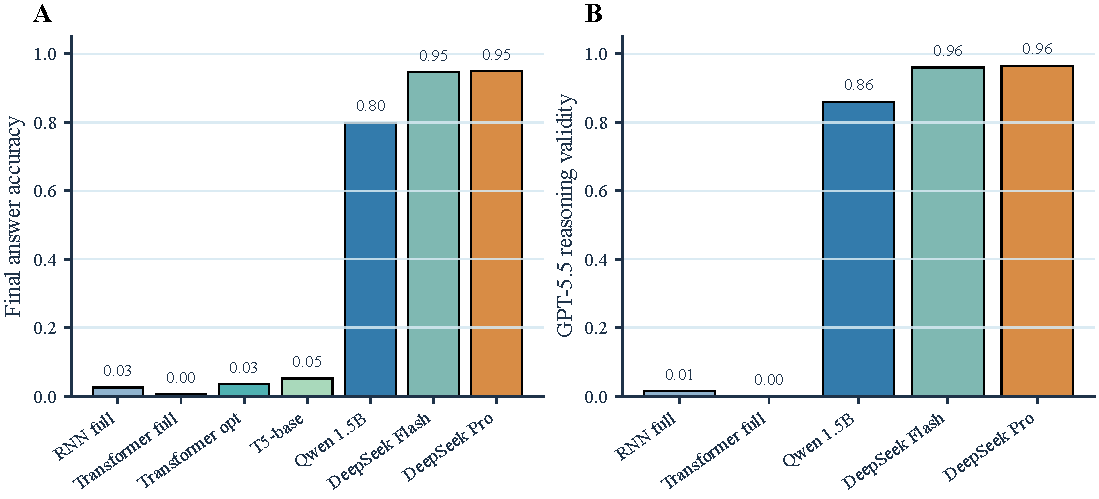
\includegraphics[width=0.95\linewidth]{main_result_panel_v8.pdf}
\caption{最终答案准确率与 GPT-5.5 推理有效率}
\label{fig:acc}
\end{figure}

\begin{figure}[H]
\centering
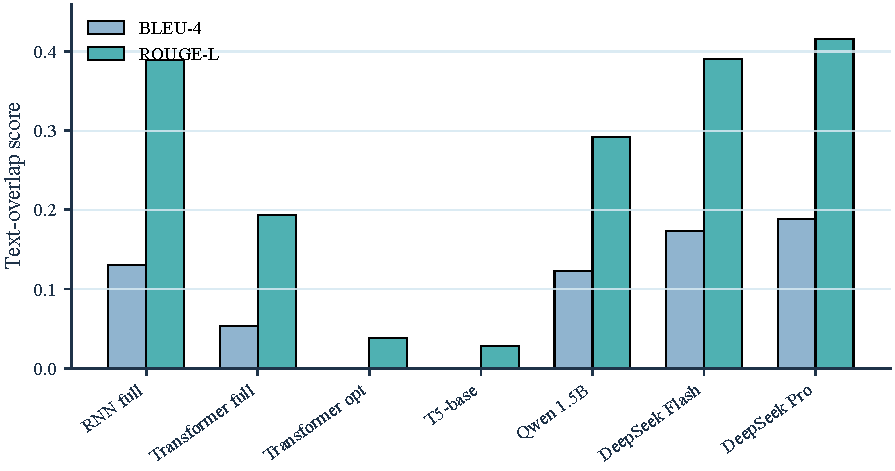
\includegraphics[width=0.95\linewidth]{automatic_metrics_panel_v8.pdf}
\caption{BLEU-4 与 ROUGE-L 辅助文本相似度指标}
\label{fig:auto}
\end{figure}

BLEU 和 ROUGE 的结果也印证了前面的担心：文本重合不等于会算题。Qwen2.5-Math-1.5B 的 BLEU-4 为 0.122963，略低于 RNN full 的 0.129968，但最终答案准确率是 0.799090，远高于 RNN full 的 0.025019。T5-base final 的 BLEU-4 为 0，最终答案准确率却达到 0.051554，高于 Transformer full 的 0.004549。也就是说，一个模型可能很会模仿参考答案的语言模板，却几乎不会算。

\subsection{任务相关指标结果}

表 \ref{tab:custom_metrics} 列出三个任务相关指标。它们比 BLEU 更直接：最终答案准确率看是否算对，格式合规率看能否被自动批改，LLM 推理有效率则检查推理过程有没有明显漏洞。

\begin{table}[H]
\centering
\caption{任务相关指标对比}
\label{tab:custom_metrics}
\small
\begin{tabular}{lccc}
\toprule
模型 & 最终答案准确率 & 格式合规率 & GPT-5.5 推理有效率 \\
\midrule
RNN full & 0.025019 & 0.903715 & 0.015 \\
Transformer full & 0.004549 & 0.245641 & 0.000 \\
Local Qwen2.5-Math-1.5B & 0.799090 & 0.953753 & 0.860 \\
DeepSeek-V4-Flash & 0.946171 & 1.000000 & 0.960 \\
DeepSeek-V4-Pro & 0.949962 & 1.000000 & 0.965 \\
\bottomrule
\end{tabular}
\end{table}

\begin{figure}[H]
\centering
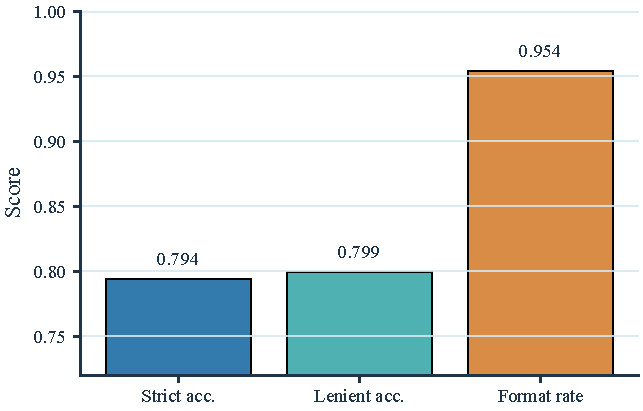
\includegraphics[width=0.68\linewidth]{qwen_strict_lenient_v8.pdf}
\caption{Qwen2.5-Math-1.5B 的 strict 与 lenient/fallback 解析结果}
\label{fig:qwen_strict}
\end{figure}

图 \ref{fig:qwen_strict} 单独展示 Qwen 的解析问题。strict 准确率为 0.794，lenient/fallback 准确率为 0.799，二者差距只有 0.005。这个结果说明，Qwen 的主要差距不是解析规则造成的；即使用更宽松的抽取方式，也只额外找回 7 道正确题。

\subsection{补充诊断}

图 \ref{fig:eqdiag} 解释了 RNN full 的一个典型问题：它很会写“像答案的答案”。RNN full 的公式覆盖率达到 0.939348，但公式执行准确率只有 0.074517；Transformer full 的公式覆盖率和公式执行准确率分别为 0.415466 和 0.034143。格式像，并不代表计算对。

\begin{figure}[H]
\centering
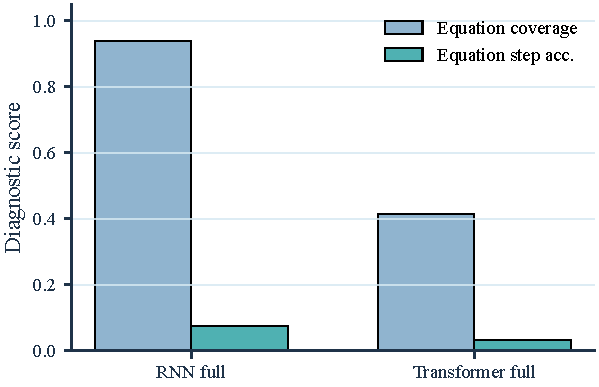
\includegraphics[width=0.58\linewidth]{diagnostic_equation_v7.pdf}
\caption{full-answer 模型的公式执行诊断}
\label{fig:eqdiag}
\end{figure}

\subsection{大模型双路径与成本}

Qwen2.5-Math-1.5B 的价值在于可本地复现，不产生 API 调用费用。DeepSeek-V4-Flash 和 DeepSeek-V4-Pro 更强，最终答案准确率和格式稳定性都更高。图 \ref{fig:cache} 显示，DeepSeek-V4-Flash 的 prompt cache hit rate 为 0.743287，DeepSeek-V4-Pro 为 0.707959。固定前缀和 warm-up 确实复用了大部分公共 prompt；由于 DeepSeek 文档说明缓存命中是 best-effort 机制，本文不对 Flash 和 Pro 的命中率差异做过强解释。

\begin{figure}[H]
\centering
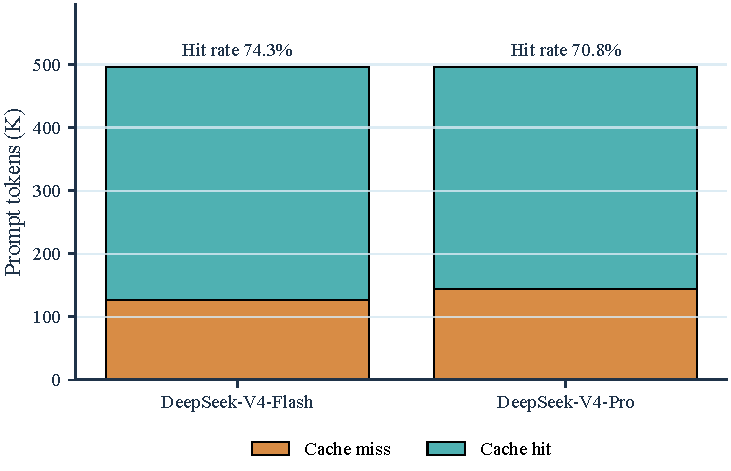
\includegraphics[width=0.72\linewidth]{deepseek_cache_v7.pdf}
\caption{DeepSeek 上下文缓存命中情况}
\label{fig:cache}
\end{figure}

按 DeepSeek 官方 2026 年 6 月价格估算，Flash 本次 1319 条测试调用约花费 0.125 美元，Pro 约花费 0.428 美元。两者准确率只差 0.0038，但 Pro 成本约为 Flash 的 3.4 倍。配对 McNemar 精确检验中，Pro 独有正确 27 题，Flash 独有正确 22 题，$p=0.568$。因此，本文只说 Pro 在本次测试中略高，不把它写成统计意义上的显著优势。

\begin{table}[H]
\centering
\caption{DeepSeek 双模型的成本与显著性对比}
\label{tab:cost}
\small
\begin{tabular}{lcccc}
\toprule
模型 & 准确率 & 估算成本（USD） & 每答对一题成本 & 缓存命中率 \\
\midrule
DeepSeek-V4-Flash & 0.946171 & 0.124653 & 0.000100 & 0.743287 \\
DeepSeek-V4-Pro & 0.949962 & 0.427717 & 0.000341 & 0.707959 \\
\bottomrule
\end{tabular}
\end{table}

\begin{figure}[H]
\centering
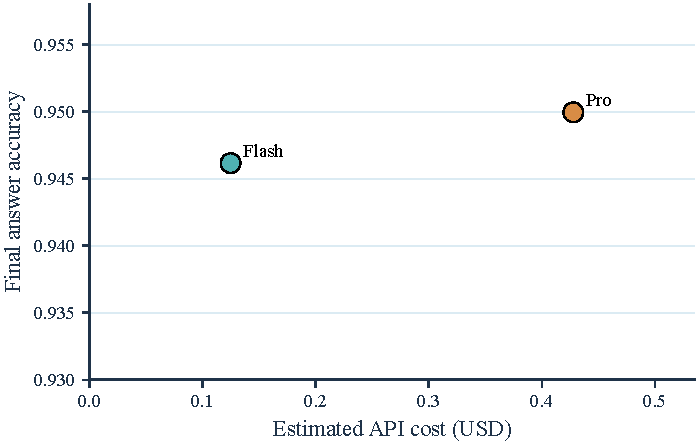
\includegraphics[width=0.68\linewidth]{cost_accuracy_v8.pdf}
\caption{DeepSeek 双模型的成本--准确率权衡}
\label{fig:cost}
\end{figure}

\subsection{LLM 抽样复核}

表 \ref{tab:judge} 是 100 条随机样本的 GPT-5.5 独立复核结果。DeepSeek-V4-Flash 和 DeepSeek-V4-Pro 的推理有效率分别为 0.960 和 0.965，本地 Qwen 为 0.860。RNN full 和 Transformer full 基本没有通过复核；它们生成的文本有时像推理，但评委很少认为它们真的讲通了。

\begin{table}[H]
\centering
\caption{随机 100 条样本的 GPT-5.5 独立评委复核结果}
\label{tab:judge}
\small
\begin{tabular}{lccccc}
\toprule
模型 & 样本数 & 平均分 & 推理有效率 & 2分比例 & 0分比例 \\
\midrule
RNN full & 100 & 0.03 & 0.015 & 0.00 & 0.97 \\
Transformer full & 100 & 0.00 & 0.000 & 0.00 & 1.00 \\
Local Qwen2.5-Math-1.5B & 100 & 1.72 & 0.860 & 0.77 & 0.05 \\
DeepSeek-V4-Flash & 100 & 1.92 & 0.960 & 0.94 & 0.02 \\
DeepSeek-V4-Pro & 100 & 1.93 & 0.965 & 0.95 & 0.02 \\
\bottomrule
\end{tabular}
\end{table}

LLM 复核很方便，但不能当成人工标注的完全替代。为避免 DeepSeek-V4-Pro 既当选手又当唯一裁判，本文主表使用 GPT-5.5 作为独立评委；原 DeepSeek-Pro 评委结果只作为早期对照。即便如此，100 条样本也只能观察主要趋势，覆盖不了全部细粒度错误。所以这个指标只用于辅助分析，不单独决定最终排名。

\section{错误分析与讨论}

\textbf{小模型的两种失败方式。}
RNN full 和 Transformer full 的准确率低，并不说明模型完全没有学到东西，而是说明它们学到的东西离“会解题”还差一层。GSM8K 要求模型同时完成英文理解、数量关系建模、多步算术和标准格式输出；对一个只用 6725 条训练样本、没有大规模预训练的小模型来说，这四件事几乎是同时从零开始学。结果就是：模型先学会了最容易模仿的部分，也就是答案的语言模板和符号外观，却没有稳定学会题目背后的计算过程。

RNN full 的失败很典型。它经常生成 \texttt{<<表达式=结果>>} 这样的 GSM8K 公式标记，格式合规率也达到 0.903715，公式覆盖率更是达到 0.939348；但公式执行准确率只有 0.074517，最终答案准确率只有 0.025019。换句话说，它像是在背标准答案的写法：知道答案里应该有公式、单位和 \texttt{\#\#\#\#}，却不知道这些数字应该如何从题目中推出来。Transformer full 的失败更靠前，它连最终答案格式都没有学稳，格式合规率只有 0.245641，很多输出里根本找不到可解析的 \texttt{\#\#\#\#} 行。

表 \ref{tab:error_examples} 给出 3 个真实错误样例。第一个样例中，RNN full 生成了 \texttt{<<...=...>>} 形式的公式标记，但表达式和结果并不匹配，最后输出 \texttt{\#\#\#\# 120}，标准答案是 18。第二个样例中，Transformer full 反复生成无意义短语，没有生成最终答案行。第三个样例中，Qwen 已经推到正确答案附近，但输出在 \texttt{\textbackslash boxed} 附近截断，导致 strict 格式解析失败。

\begin{table}[H]
\centering
\caption{典型错误样例}
\label{tab:error_examples}
\small
\setlength{\tabcolsep}{4pt}
\begin{tabular}{>{\raggedright\arraybackslash}p{0.23\textwidth}>{\raggedright\arraybackslash}p{0.12\textwidth}>{\raggedright\arraybackslash}p{0.43\textwidth}>{\raggedright\arraybackslash}p{0.15\textwidth}}
\toprule
题目简述 & 标准答案 & 模型输出片段 & 错误类型 \\
\midrule
鸭蛋每日收入题 & \texttt{\#\#\#\# 18} & RNN full 输出 \texttt{<<12*12=12>>}、\texttt{<<12*12=120>>}，最后给出 \texttt{\#\#\#\# 120}。 & 公式格式像，但计算错 \\
房屋翻修利润题 & \texttt{\#\#\#\# 70000} & Transformer full 反复生成 ``the price of the price''，没有输出 \texttt{\#\#\#\#} 最终答案行。 & 格式不可解析 \\
自行车打气收费题 & \texttt{\#\#\#\# 5} & Qwen 推理到 500 cents = 5 dollars，但结尾停在 \texttt{\textbackslash boxed}，strict 解析不到最终答案。 & 推理接近正确，但格式截断 \\
\bottomrule
\end{tabular}
\end{table}

除了个别样例，我们还统计了 Qwen 与两个 DeepSeek 模型的错误类型，结果见图 \ref{fig:error_breakdown}。Qwen 的错误主要是最终数字错误（204 条）和缺少明确最终答案标记（54 条），另有 7 条属于“strict 抽不到但 fallback 抽对”。DeepSeek-Flash 和 DeepSeek-Pro 的格式合规率均为 1.0，剩余错误主要是答案本身错误，分别为 71 条和 66 条。这说明大模型后 5\% 左右的错误已经不是模板失败，而是题意理解、边界条件或多步计算中的真实错误。

\begin{figure}[H]
\centering
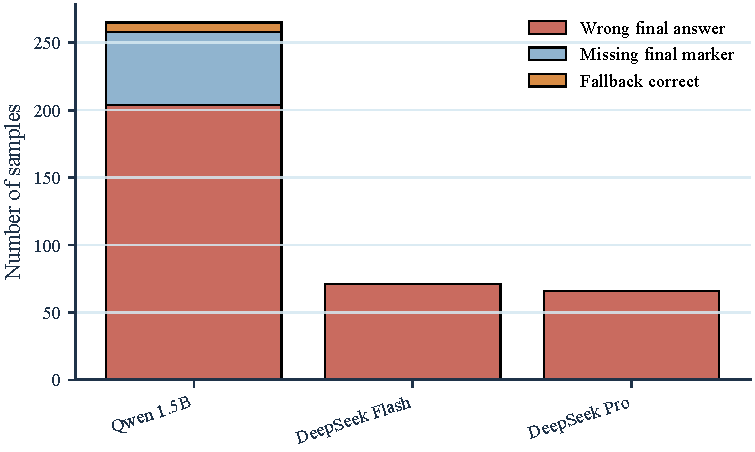
\includegraphics[width=0.74\linewidth]{error_breakdown_v8.pdf}
\caption{Qwen 与 DeepSeek 的错误类型统计}
\label{fig:error_breakdown}
\end{figure}

\textbf{只改输出目标，不会自动带来推理能力。}
final-only 模型把目标压缩到最终答案，格式合规率立刻变成 1.0，但准确率几乎没有本质提升。这个结果很关键：如果低分主要来自格式解析，那么只输出 \texttt{\#\#\#\# answer} 后准确率应该明显上涨；但实际并没有。Transformer final optimized 是自实现模型中的最佳结果，最终答案准确率也只有 0.034875。它比 full-answer Transformer 好一些，但仍然接近随机猜数。由此可以判断，小模型的瓶颈不是“不会按格式输出”，而是内部没有形成可靠的多步算术推理能力。

\textbf{预训练有用，但不够。}
T5-base 相比自实现 Transformer 有提升，准确率达到 0.051554。这个提升说明预训练确实提供了更好的语言建模基础，至少让模型更容易理解题目和生成稳定输出；但只做 final-only 微调、模型规模又有限，它仍不能稳定解决 GSM8K 的多步推理。这个结果也解释了为什么 Qwen 和 DeepSeek 会出现数量级提升：它们并不是只靠“更会生成文本”，而是已经在大规模语料和数学解题链上获得了更强的语言理解与计算模式。

\textbf{大模型为什么强？}
Qwen2.5-Math-1.5B 是数学专项模型，训练中接触过大量解题链，因此即使只有 1.5B 参数，也能在本地跑到 0.799090。DeepSeek 系列更强，Flash 和 Pro 分别达到 0.946171 和 0.949962，格式合规率均为 1.0。但二者只差约 5 道题，统计检验不支持“Pro 显著强于 Flash”的说法。结合成本，Flash 更适合成本敏感场景；Pro 是否值得额外成本，需要看任务是否真的需要那一点点单次精度优势。这个对比也把全文的主线收束回来：在数学问答里，文本重合指标只能说明模型是否像参考答案，最终数字和推理有效性才更接近“是否真的会算”。

\section{结论}

同一批 GSM8K 测试题，把模型差距拉得很开。我们得到三个结论。

\begin{itemize}
  \item \textbf{模型规模和预训练显著提高上限。} 从零训练的小模型最终答案准确率低于 0.04；1.5B 的数学专项模型 Qwen2.5-Math-1.5B 达到 0.799；DeepSeek-V4-Pro 和 Flash 则接近 0.95。
  \item \textbf{BLEU/ROUGE 会误导数学问答评测。} RNN full 的 BLEU-4 略高于 Qwen，但最终答案准确率相差 30 倍以上。数学问答必须看最终数字和推理过程。
  \item \textbf{本地部署和云端 API 各有位置。} Qwen2.5-Math-1.5B 可以离线复现，适合成本和隐私敏感场景；DeepSeek-Flash 以明显更低成本接近 Pro；Pro 在本次测试中略高，但优势没有通过配对显著性检验。
\end{itemize}

实验仍有局限。Qwen LoRA 微调脚本已经补充到工程中，但由于本机环境首次加载模型耗时较长，最终论文主表仍采用已完整跑完的 few-shot 结果；DeepSeek 的缓存命中率超过 70\%，但没有系统比较不同 prompt 结构的影响；GPT-5.5 评委比 DeepSeek 自评更独立，但仍不能完全替代人工标注。还有一个值得继续追问的问题：DeepSeek-Pro 仍有约 5\% 的题目算错，这些错误到底来自计算、推理，还是题目表述本身？后续可以加入 SVAMP、MultiArith 等数据集，并对 prompt 数量、温度、LoRA 微调轮数和人工评委一致性做更细的消融。

\appendix
\section{大模型提示词模板}

Qwen 与 DeepSeek 都使用少量示例引导模型按步骤计算，并要求最终答案使用统一格式。DeepSeek API 实验把示例部分作为固定前缀，以提高上下文缓存命中率。简化模板如下：

\begin{verbatim}
You are a precise GSM8K math solver.
Solve arithmetic word problems carefully.
Show concise step-by-step arithmetic.
The final line must be exactly: #### number

Example 1:
Question: A store has 12 pencils. It buys 8 more pencils
and then sells 5. How many pencils are left?
Answer:
The store has 12 + 8 = 20 pencils after buying more.
After selling 5, it has 20 - 5 = 15 pencils left.
#### 15

Now solve:
Question: {question}
Answer:
\end{verbatim}

\clearpage
\begin{thebibliography}{99}

\bibitem{cobbe2021gsm8k}
Cobbe K, Kosaraju V, Bavarian M, et al.
Training Verifiers to Solve Math Word Problems.
arXiv:2110.14168, 2021.
\url{https://arxiv.org/abs/2110.14168}

\bibitem{vaswani2017attention}
Vaswani A, Shazeer N, Parmar N, et al.
Attention Is All You Need.
Advances in Neural Information Processing Systems, 2017.
\url{https://arxiv.org/abs/1706.03762}

\bibitem{raffel2020t5}
Raffel C, Shazeer N, Roberts A, et al.
Exploring the Limits of Transfer Learning with a Unified Text-to-Text Transformer.
Journal of Machine Learning Research, 2020.
\url{https://arxiv.org/abs/1910.10683}

\bibitem{yang2024qwen25math}
Yang A, Li B, Hui B, et al.
Qwen2.5-Math Technical Report: Toward Mathematical Expert Model via Self-Improvement.
arXiv:2409.12122, 2024.
\url{https://arxiv.org/abs/2409.12122}

\bibitem{deepseekprice}
DeepSeek.
Models \& Pricing.
\url{https://api-docs.deepseek.com/quick_start/pricing}

\bibitem{deepseekcache}
DeepSeek.
Context Caching.
\url{https://api-docs.deepseek.com/guides/kv_cache}

\end{thebibliography}

\end{document}
